\documentclass[12pt,a4paper]{article}

% ============================================================
% Pakete
% ============================================================
\usepackage[utf8]{inputenc}
\usepackage[T1]{fontenc}
\usepackage[ngerman]{babel}
\usepackage{amsmath, amssymb, amsthm}
\usepackage{mathtools}
\usepackage{geometry}
\usepackage{graphicx}
\usepackage{xcolor}
\usepackage{booktabs}
\usepackage{array}
\usepackage{fancyhdr}
\usepackage{hyperref}
\usepackage{circuitikz}
\usetikzlibrary{decorations.pathreplacing, calc}
\usepackage{pgfplots}
\usepackage{siunitx}
\usepackage{tcolorbox}
\usepackage{enumitem}
\usepackage{float}
\usepackage{caption}
\usepackage{subcaption}
\usepackage{titlesec}
\usepackage{lmodern}

\pgfplotsset{compat=1.18}
\geometry{left=2.5cm, right=2.5cm, top=3cm, bottom=3cm, headheight=25pt}

% ============================================================
% Farben (FH Vorarlberg Corporate Design)
% ============================================================
\definecolor{fhgelb}{RGB}{255, 200, 0}
\definecolor{fhdunkel}{RGB}{40, 40, 40}
\definecolor{fhblau}{RGB}{0, 80, 155}
\definecolor{kastenhintergrund}{RGB}{240, 248, 255}
\definecolor{ergebnisfarbe}{RGB}{220, 240, 220}

% ============================================================
% tcolorbox Styles
% ============================================================
\tcbset{
  ergebnis/.style={
    colback=ergebnisfarbe,
    colframe=fhblau,
    fonttitle=\bfseries,
    title=Ergebnis,
    boxrule=1pt,
    arc=4pt
  },
  hinweis/.style={
    colback=kastenhintergrund,
    colframe=fhblau!60,
    fonttitle=\bfseries,
    boxrule=0.8pt,
    arc=4pt
  },
  formel/.style={
    colback=gray!8,
    colframe=fhdunkel!40,
    boxrule=0.6pt,
    arc=3pt
  }
}

% ============================================================
% Kopf- und Fußzeile
% ============================================================
\pagestyle{fancy}
\fancyhf{}
\fancyhead[L]{\textbf{Messschaltungen und Sensorik}}
\fancyhead[R]{Stefan Bonerz / Christoph Stüttler}
\fancyfoot[C]{\thepage}
\renewcommand{\headrulewidth}{1.5pt}
\renewcommand{\headrule}{\hbox to\headwidth{%
  \color{fhgelb}\leaders\hrule height \headrulewidth\hfill}}

% ============================================================
% Abschnittsstile
% ============================================================
\titleformat{\section}[block]
  {\large\bfseries\color{fhblau}}
  {\thesection}{1em}{}[\titlerule]

\titleformat{\subsection}[block]
  {\normalsize\bfseries\color{fhdunkel}}
  {\thesubsection}{1em}{}

% ============================================================
% Nützliche Makros
% ============================================================
\newcommand{\laplace}{s}            % Laplace-Variable
\newcommand{\jw}{j\omega}
\newcommand{\abs}[1]{\left|#1\right|}
\newcommand{\Tf}{\hat{T}}           % Übertragungsfunktion
\newcommand{\Z}[1]{Z_{#1}}
\newcommand{\Rone}{R_1}
\newcommand{\Rtwo}{R_2}
\newcommand{\Rthree}{R_3}
\newcommand{\Rfour}{R_4}
\newcommand{\Cone}{C_1}
\newcommand{\Ctwo}{C_2}

% ============================================================
% DOKUMENT
% ============================================================
\begin{document}

% ============================================================
% Titelseite
% ============================================================
\begin{titlepage}
  \centering
  \vspace*{1cm}
  {\Huge\bfseries\color{fhblau} Messschaltungen und Sensorik\par}
  \vspace{0.5cm}
  \rule{\linewidth}{2pt}
  \vspace{0.5cm}
  {\LARGE\bfseries Projekt: Frequenzabhängige\\[4pt]
   OP-Verstärkerschaltung (PID-Regler)\par}
  \vspace{0.5cm}
  \rule{\linewidth}{1pt}
  \vspace{1.5cm}
  {\large Stefan Bonerz \quad/\quad Christoph Stüttler\par}
  \vspace{0.5cm}
  {\large FH Vorarlberg --- University of Applied Sciences\par}
  \vspace{0.5cm}
  {\large Abgabetermin: 14.\,Juni\,2026\par}
  \vfill
  {\normalsize\color{gray} Dokumentation erstellt im Rahmen des Moduls\\
   \textit{Messschaltungen und Sensorik}}
\end{titlepage}

% ============================================================
% Inhaltsverzeichnis
% ============================================================
\tableofcontents
\newpage

% ============================================================
\section{Einleitung}
% ============================================================

Mit invertierenden Operationsverstärker-Schaltungen lassen sich frequenzabhängige
Verstärkungen realisieren, indem die Widerstände $R_1$ und $R_2$ der klassischen
Invertier-Grundschaltung durch allgemeine Impedanzen $Z_1$ und $Z_2$ ersetzt werden.
Durch geeignete Wahl dieser Impedanzen können einfache Filter (Tief-, Hochpass) oder ---
wie in diesem Projekt --- analoge PID-Regler konstruiert werden.

\textbf{Ziel dieser Dokumentation} ist die vollständige analytische Herleitung der
Übertragungsfunktion der vorgegebenen Schaltung sowie die Bestimmung der Bauteilwerte,
sodass der geforderte Amplitudengang entsteht. Die anschließende Simulation in LTSpice
dient der Verifikation.

% ============================================================
\section{Gegebene Größen und Schaltungsstruktur}
% ============================================================

\subsection{Vorgegebene Bauteilwerte}

\begin{table}[H]
  \centering
  \caption{Vorgegebene und gesuchte Bauteilwerte}
  \begin{tabular}{lll}
    \toprule
    Bauteil & Wert & Status \\
    \midrule
    $C_2$ & $0{,}1\,\mu\text{F}$ & vorgegeben \\
    $C_1$ & ? & gesucht \\
    $R_1, R_2, R_3, R_4$ & ? & gesucht ($1\,\text{k}\Omega < R < 1\,\text{M}\Omega$) \\
    OP-Amp & ADTL082 & vorgegeben \\
    \bottomrule
  \end{tabular}
\end{table}

\subsection{Geforderte Eckfrequenzen aus dem Amplitudengang}

Aus dem geforderten Bode-Diagramm (Amplitudengang) lassen sich vier charakteristische
Kreisfrequenzen ablesen:

\[
  \omega_1 = 62\,\frac{\text{rad}}{\text{s}}, \quad
  \omega_2 = 620\,\frac{\text{rad}}{\text{s}}, \quad
  \omega_3 = 6200\,\frac{\text{rad}}{\text{s}}, \quad
  \omega_4 = 62000\,\frac{\text{rad}}{\text{s}}
\]

Diese entsprechen den vier Pol-/Nullstellen-Frequenzen der Übertragungsfunktion.

\subsection{Schaltungsstruktur}

Die Schaltung ist eine invertierende OP-Schaltung. Die Impedanz $Z_1$ im
Eingangsast besteht aus der Reihenschaltung von $C_1$ und $R_2$, parallel dazu liegt
$R_1$. Die Rückkopplungsimpedanz $Z_2$ besteht aus der Parallelschaltung von
($C_2$ in Reihe mit $R_4$) und $R_3$.

\begin{figure}[H]
  \centering
  \begin{circuitikz}[scale=1.0, transform shape]

    % ── Koordinaten ─────────────────────────────────────────────
    \coordinate (uestart) at (-1.5, 0);   % langer Eingangspin
    \coordinate (ue)      at (0,    0);   % Verzweigungspunkt Z1
    \coordinate (vm)      at (3.5,  0);   % virtueller Massepunkt = neg. OP-Eingang

    % ── Eingangsleitung (lang) ───────────────────────────────────
    \draw (uestart) node[left]{$u_e$} to[short] (ue);

    % ── Z1: oberer Zweig R1 (ue --> vm) ─────────────────────────
    \draw (ue) to[R, l=$R_1$] (vm);

    % ── Z1: unterer Zweig C1--R2 in Serie (ue --> vm) ───────────
    \draw (ue)
      to[short] (0,-1.8)
      to[C, l=$C_1$] (1.75,-1.8)
      to[R, l=$R_2$] (3.5,-1.8)
      to[short] (vm);

    % Klammer Z1
    \draw[decorate, decoration={brace, mirror, amplitude=6pt}, color=fhblau]
      (0,-2.5) -- (3.5,-2.5) node[midway, below=8pt]{$Z_1$};

    % ── OP-Amp  (inv input up → „−" oben, „+" unten) ─────────────
    % Mit noinv input up ist „+" oben und „−" unten → wir wollen
    % aber „−" oben. Daher verwenden wir den Standard-OP (inv unten)
    % und spiegeln ihn vertikal mit yscale=-1:
    \node[op amp, yscale=1, anchor=-] (op) at (5.5, 0) {};

    % Verbindung vm --> neg. Eingang (oben)
    \draw (vm) to[short, -*] (op.-);

    % pos. Eingang (unten) --> GND
    \draw (op.+) to[short] ++(0,-0.1) node[ground]{};

    % ── Z2: Rückkopplung (Ausgang --> neg. Eingang) ───────────────
    \coordinate (outR) at ($(op.out) + (0.5,0)$);

    % Ausgangs-Stub + Ausgangspin
    \draw (op.out) to[short, -*] (outR);
    \draw (outR)   to[short]     ++(0.8,0) node[right]{$u_a$};

    % Unterer Rückkopplungsast: R3 allein, über y=2.0
    \draw (outR)
      to[short] (outR |- 0,2.0)
      to[R, l=$R_3$] (vm |- 0,2.0)
      to[short] (vm);

    % Oberer Rückkopplungsast: R4--C2 in Serie (R4 links, C2 rechts), über y=3.4
    \draw (outR |- 0,2.0)
      to[short] (outR |- 0,3.4)
      to[R, l=$R_4$] ($(vm |- 0,3.4)!0.5!(outR |- 0,3.4)$)
      to[C, l=$C_2$] (vm |- 0,3.4)
      to[short] (vm |- 0,2.0);

    % Klammer Z2
    \draw[decorate, decoration={brace, amplitude=6pt}, color=fhblau]
      (vm |- 0,4.1) -- (outR |- 0,4.1)
      node[midway, above=8pt]{$Z_2$};

  \end{circuitikz}
  \caption{Invertierende OP-Schaltung: $Z_1 = R_1 \parallel (C_1 + R_2)$,\;
           $Z_2 = R_3 \parallel (R_4 + C_2)$}
\end{figure}

% ============================================================
\section{Aufgabe 1: Herleitung der Übertragungsfunktion}
% ============================================================
 
\subsection{Grundprinzip der invertierenden OP-Schaltung}
 
Für eine invertierende OP-Schaltung mit idealem Operationsverstärker gelten die
\textbf{zwei goldenen Regeln}:
\begin{enumerate}
  \item Die Spannung am invertierenden Eingang entspricht der am nicht-invertierenden
        Eingang. Da $u_+ = 0\,\text{V}$ (GND), gilt $u_- = 0\,\text{V}$ (virtuelle Masse).
  \item Es fließt kein Strom in die Eingänge des OP: $i_+ = i_- = 0$.
\end{enumerate}
 
Aus der Knotenregel am invertierenden Eingang (virtuelle Masse) folgt:
\[
  \frac{u_e - 0}{Z_1} + \frac{u_a - 0}{Z_2} = 0
  \quad \Longrightarrow \quad
  \frac{u_e}{Z_1} = -\frac{u_a}{Z_2}
\]
 
Umformen ergibt die allgemeine Übertragungsfunktion:
 
\begin{tcolorbox}[formel]
\[
  T(s) = \frac{U_a(s)}{U_e(s)} = -\frac{Z_2(s)}{Z_1(s)}
\]
\end{tcolorbox}
 
Das Minuszeichen bedeutet Signalumkehr (Invertierung). Im Amplitudengang $|T(j\omega)|$
entfällt es.
 
% ------------------------------------------------------------
\subsection{Berechnung der Eingangsimpedanz $Z_1$}
% ------------------------------------------------------------
 
Die Impedanz $Z_1$ besteht aus zwei parallelen Zweigen:
\begin{itemize}
  \item Oberer Zweig: $R_1$ allein
  \item Unterer Zweig: $C_1$ und $R_2$ in Serie
\end{itemize}
 
\[
  Z_1 = R_1 \;\parallel\; \left(\frac{1}{sC_1} + R_2\right)
\]
 
\subsubsection*{Schritt 1: Serienimpedanz des unteren Zweiges}
 
\[
  Z_{C_1R_2} = \frac{1}{sC_1} + R_2
             = \frac{1 + sC_1 R_2}{sC_1}
\]
 
\subsubsection*{Schritt 2: Parallelschaltung}
 
\[
  Z_1 = \frac{R_1 \cdot Z_{C_1R_2}}{R_1 + Z_{C_1R_2}}
\]
 
Zähler:
\[
  R_1 \cdot Z_{C_1R_2}
  = R_1 \cdot \frac{1 + sC_1 R_2}{sC_1}
\]
 
Nenner:
\[
  R_1 + Z_{C_1R_2}
  = R_1 + \frac{1 + sC_1 R_2}{sC_1}
  = \frac{sC_1 R_1 + 1 + sC_1 R_2}{sC_1}
  = \frac{1 + sC_1(R_1 + R_2)}{sC_1}
\]
 
Division (gemeinsamer Faktor $sC_1$ kürzt sich):
\[
  Z_1
  = \frac{R_1 \cdot \dfrac{1 + sC_1 R_2}{sC_1}}{\dfrac{1 + sC_1(R_1+R_2)}{sC_1}}
  = R_1 \cdot \frac{1 + sC_1 R_2}{1 + sC_1(R_1 + R_2)}
\]
 
\begin{tcolorbox}[ergebnis]
\[
  \boxed{Z_1 = R_1 \cdot \frac{1 + sC_1 R_2}{1 + sC_1(R_1 + R_2)}}
\]
\end{tcolorbox}
 
% ------------------------------------------------------------
\subsection{Berechnung der Rückkopplungsimpedanz $Z_2$}
% ------------------------------------------------------------
 
Die Impedanz $Z_2$ besteht aus zwei parallelen Zweigen:
\begin{itemize}
  \item Unterer Zweig: $R_3$ allein
  \item Oberer Zweig: $R_4$ und $C_2$ in Serie
\end{itemize}
 
\[
  Z_2 = R_3 \;\parallel\; \left(R_4 + \frac{1}{sC_2}\right)
\]
 
\subsubsection*{Schritt 1: Serienimpedanz des oberen Zweiges}
 
\[
  Z_{R_4C_2} = R_4 + \frac{1}{sC_2}
             = \frac{sC_2 R_4 + 1}{sC_2}
             = \frac{1 + sC_2 R_4}{sC_2}
\]
 
\subsubsection*{Schritt 2: Parallelschaltung}
 
\[
  Z_2 = \frac{R_3 \cdot Z_{R_4C_2}}{R_3 + Z_{R_4C_2}}
\]
 
Zähler:
\[
  R_3 \cdot Z_{R_4C_2}
  = R_3 \cdot \frac{1 + sC_2 R_4}{sC_2}
\]
 
Nenner:
\[
  R_3 + Z_{R_4C_2}
  = R_3 + \frac{1 + sC_2 R_4}{sC_2}
  = \frac{sC_2 R_3 + 1 + sC_2 R_4}{sC_2}
  = \frac{1 + sC_2(R_3 + R_4)}{sC_2}
\]
 
Division ($sC_2$ kürzt sich):
\[
  Z_2
  = \frac{R_3 \cdot \dfrac{1 + sC_2 R_4}{sC_2}}{\dfrac{1 + sC_2(R_3+R_4)}{sC_2}}
  = R_3 \cdot \frac{1 + sC_2 R_4}{1 + sC_2(R_3 + R_4)}
\]
 
\begin{tcolorbox}[ergebnis]
\[
  \boxed{Z_2 = R_3 \cdot \frac{1 + sC_2 R_4}{1 + sC_2(R_3 + R_4)}}
\]
\end{tcolorbox}
 
% ------------------------------------------------------------
\subsection{Gesamte Übertragungsfunktion $T(s) = -Z_2/Z_1$}
% ------------------------------------------------------------
 
\[
  T(s) = -\frac{Z_2}{Z_1}
        = -\frac{R_3 \cdot \dfrac{1 + sC_2 R_4}{1 + sC_2(R_3 + R_4)}}
               {R_1 \cdot \dfrac{1 + sC_1 R_2}{1 + sC_1(R_1 + R_2)}}
\]
 
Durch Kürzen des Doppelbruchs (Zähler $\div$ Nenner):
 
\[
  T(s) = -\frac{R_3}{R_1}
         \cdot \frac{1 + sC_2 R_4}{1 + sC_2(R_3 + R_4)}
         \cdot \frac{1 + sC_1(R_1 + R_2)}{1 + sC_1 R_2}
\]
 
Da für den Amplitudengang nur $|T|$ relevant ist, entfällt das Minuszeichen:
 
\begin{tcolorbox}[ergebnis, title={\"Ubertragungsfunktion des PID-Reglers}]
\[
  \boxed{|T(s)| = \frac{R_3}{R_1}
         \cdot \frac{1 + sC_2 R_4}{1 + sC_2(R_3 + R_4)}
         \cdot \frac{1 + sC_1(R_1 + R_2)}{1 + sC_1 R_2}}
\]
Dies stimmt mit dem gegebenen Kontrollergebnis überein. $\checkmark$
\end{tcolorbox}
 
% ------------------------------------------------------------
\subsection{Interpretation der vier Terme}
% ------------------------------------------------------------
 
Die Übertragungsfunktion enthält vier frequenzabhängige Terme plus den
Gleichspannungsfaktor:
 
\begin{enumerate}[label=\textbf{\arabic{enumi}.}]
  \item \textbf{Gleichspannungsverstärkung} (frequenzunabhängig):
    \[
      K_0 = \frac{R_3}{R_1}
    \]
 
  \item \textbf{Pol bei $\omega_1$} --- Tiefpass-Term im Nenner von $Z_1$:
    \[
      \frac{1}{1 + sC_1(R_1+R_2)}
      \qquad \Rightarrow \qquad
      \omega_1 = \frac{1}{C_1(R_1+R_2)}
    \]
    Knick \textbf{nach unten} ($-20\,\text{dB/Dek.}$) bei $\omega_1$.
 
  \item \textbf{Nullstelle bei $\omega_2$} --- Zähler-Term aus $Z_1$:
    \[
      1 + sC_1 R_2
      \qquad \Rightarrow \qquad
      \omega_2 = \frac{1}{C_1 R_2}
    \]
    Knick \textbf{nach oben} ($+20\,\text{dB/Dek.}$) bei $\omega_2$.
    Da $R_2 < R_1+R_2$ folgt $\omega_2 > \omega_1$. $\checkmark$
 
  \item \textbf{Pol bei $\omega_3$} --- Tiefpass-Term im Nenner von $Z_2$:
    \[
      \frac{1}{1 + sC_2(R_3+R_4)}
      \qquad \Rightarrow \qquad
      \omega_3 = \frac{1}{C_2(R_3+R_4)}
    \]
    Knick \textbf{nach unten} ($-20\,\text{dB/Dek.}$) bei $\omega_3$.
 
  \item \textbf{Nullstelle bei $\omega_4$} --- Zähler-Term aus $Z_2$:
    \[
      1 + sC_2 R_4
      \qquad \Rightarrow \qquad
      \omega_4 = \frac{1}{C_2 R_4}
    \]
    Knick \textbf{nach oben} ($+20\,\text{dB/Dek.}$) bei $\omega_4$.
    Da $R_4 < R_3+R_4$ folgt $\omega_4 > \omega_3$. $\checkmark$
\end{enumerate}
 
% ============================================================
\section{Aufgabe 2: Bestimmung der Bauteilwerte}
% ============================================================
 
\subsection{Zuordnung der Eckfrequenzen zum Amplitudengang}
 
Aus dem geforderten Bode-Diagramm (Amplitudengang des PID) lassen sich vier
Eckfrequenzen mit ihren Knickrichtungen ablesen:
 
\begin{table}[H]
  \centering
  \caption{Eckfrequenzen und ihre Zuordnung}
  \begin{tabular}{cccc}
    \toprule
    Kreisfrequenz & Knick & Typ & Term \\
    \midrule
    $\omega_1 = 62\,\text{rad/s}$    & $-20\,\text{dB/Dek.}$ & Pol (Nenner)        & $1 + sC_1(R_1+R_2)$ \\
    $\omega_2 = 620\,\text{rad/s}$   & $+20\,\text{dB/Dek.}$ & Nullstelle (Zähler) & $1 + sC_1 R_2$ \\
    $\omega_3 = 6200\,\text{rad/s}$  & $-20\,\text{dB/Dek.}$ & Pol (Nenner)        & $1 + sC_2(R_3+R_4)$ \\
    $\omega_4 = 62000\,\text{rad/s}$ & $+20\,\text{dB/Dek.}$ & Nullstelle (Zähler) & $1 + sC_2 R_4$ \\
    \bottomrule
  \end{tabular}
\end{table}
 
\begin{tcolorbox}[hinweis, title=Hinweis zur Zuordnung]
Der Amplitudengang startet bei $|T(0)| = R_3/R_1$ und fällt bei $\omega_1$ ab
$\Rightarrow$ Pol (Nenner-Term, $-20\,\text{dB/Dek.}$). Bei $\omega_2$ steigt er
wieder $\Rightarrow$ Nullstelle (Zähler-Term, $+20\,\text{dB/Dek.}$). Dasselbe
Muster wiederholt sich im Rückkopplungszweig: $\omega_3$ ist ein Pol, $\omega_4$
eine Nullstelle. Die Bedingung $\omega_{\text{Pol}} < \omega_{\text{Nullstelle}}$
ist jeweils erfüllt, da $R_1+R_2 > R_2$ und $R_3+R_4 > R_4$.
\end{tcolorbox}
 
\subsection{Gleichungssystem aus den Eckfrequenzen}
 
Die vier Eckfrequenz-Bedingungen liefern vier Gleichungen:
 
\begin{align}
  \frac{1}{C_1(R_1 + R_2)} &= \omega_1 = 62    \label{eq:omega1} \\[6pt]
  \frac{1}{C_1 \, R_2}      &= \omega_2 = 620   \label{eq:omega2} \\[6pt]
  \frac{1}{C_2(R_3 + R_4)}  &= \omega_3 = 6200  \label{eq:omega3} \\[6pt]
  \frac{1}{C_2 \, R_4}       &= \omega_4 = 62000 \label{eq:omega4}
\end{align}
 
% ------------------------------------------------------------
\subsection{Berechnung von $C_1$, $R_1$, $R_2$}
% ------------------------------------------------------------
 
\subsubsection*{Schritt 1: Verhältnis $\omega_2 / \omega_1$ liefert $R_1/R_2$}
 
Gleichung~\eqref{eq:omega2} durch Gleichung~\eqref{eq:omega1}:
 
\[
  \frac{\omega_2}{\omega_1}
  = \frac{\dfrac{1}{C_1 R_2}}{\dfrac{1}{C_1(R_1+R_2)}}
  = \frac{C_1(R_1+R_2)}{C_1 R_2}
  = 1 + \frac{R_1}{R_2}
\]
 
\[
  \frac{R_1}{R_2}
  = \frac{\omega_2}{\omega_1} - 1
  = \frac{620}{62} - 1
  = 10 - 1
  = 9
  \quad \Longrightarrow \quad
  \boxed{R_1 = 9\,R_2}
\]
 
\subsubsection*{Schritt 2: Wahl von $R_2$, Berechnung von $C_1$}
 
$R_2$ frei wählbar im Bereich $1\,\text{k}\Omega < R_2 < 1\,\text{M}\Omega$.
Aus Gleichung~\eqref{eq:omega2}:
 
\[
  C_1 = \frac{1}{\omega_2 \cdot R_2}
\]
 
Wir wählen $R_2 = 16\,\text{k}\Omega$ (E24-Normwert), dann:
 
\[
  C_1 = \frac{1}{620 \cdot 16\,000}
      = \frac{1}{9{,}92 \times 10^{6}}
      \approx 1{,}008 \times 10^{-7}\,\text{F}
      \approx 100\,\text{nF}
\]
 
Wähle: $\boxed{C_1 = 100\,\text{nF}}$
 
\subsubsection*{Schritt 3: Rückrechnung exakter $R_2$ und $R_1$}
 
Mit $C_1 = 100\,\text{nF}$ exakt aus Gl.~\eqref{eq:omega2}:
\[
  R_2 = \frac{1}{\omega_2 \cdot C_1}
      = \frac{1}{620 \cdot 10^{-7}}
      = \frac{1}{6{,}2 \times 10^{-5}}
      \approx 16\,129\,\Omega
      \approx 16{,}1\,\text{k}\Omega
\]
 
\[
  R_1 = 9 \cdot R_2 = 9 \cdot 16\,129 \approx 145\,161\,\Omega \approx 145\,\text{k}\Omega
\]
 
\subsubsection*{Schritt 4: Verifikation}
 
\[
  \omega_1 = \frac{1}{C_1(R_1+R_2)}
           = \frac{1}{10^{-7} \cdot (145\,161 + 16\,129)}
           = \frac{1}{10^{-7} \cdot 161\,290}
           = \frac{1}{1{,}6129 \times 10^{-2}}
           \approx 62{,}0\,\frac{\text{rad}}{\text{s}} \checkmark
\]
\[
  \omega_2 = \frac{1}{C_1 \cdot R_2}
           = \frac{1}{10^{-7} \cdot 16\,129}
           = \frac{1}{1{,}6129 \times 10^{-3}}
           \approx 620\,\frac{\text{rad}}{\text{s}} \checkmark
\]
 
\begin{tcolorbox}[ergebnis, title={Ergebnis f\"{u}r $C_1$, $R_1$, $R_2$}]
\[
  C_1 = 100\,\text{nF}, \qquad
  R_2 \approx 16{,}1\,\text{k}\Omega \;\widehat{=}\; 16\,\text{k}\Omega, \qquad
  R_1 \approx 145\,\text{k}\Omega \;\widehat{=}\; 150\,\text{k}\Omega
\]
\end{tcolorbox}
 
% ------------------------------------------------------------
\subsection{Berechnung von $C_2$, $R_3$, $R_4$}
% ------------------------------------------------------------
 
\subsubsection*{Schritt 1: Prüfung ob $C_2 = 0{,}1\,\mu\text{F}$ zulässig ist}
 
Der vorgeschlagene Wert $C_2 = 0{,}1\,\mu\text{F}$ wird zuerst geprüft.
Aus Gleichung~\eqref{eq:omega4} (Nullstelle bei $\omega_4 = 62000$):
 
\[
  R_4 = \frac{1}{\omega_4 \cdot C_2}
      = \frac{1}{62000 \cdot 0{,}1 \times 10^{-6}}
      = \frac{1}{6{,}2 \times 10^{-3}}
      \approx 161\,\Omega
      \quad \Rightarrow \quad \text{\textbf{Verletzt } } R > 1\,\text{k}\Omega!
\]
 
Aus Gleichung~\eqref{eq:omega3} (Pol bei $\omega_3 = 6200$):
\[
  R_3 + R_4 = \frac{1}{\omega_3 \cdot C_2}
            = \frac{1}{6200 \cdot 0{,}1 \times 10^{-6}}
            \approx 1613\,\Omega
  \quad \Rightarrow \quad
  R_3 = 1613 - 161 = 1452\,\Omega
  \quad \Rightarrow \quad \text{\textbf{ebenfalls verletzt!}}
\]
 
$C_2 = 0{,}1\,\mu\text{F}$ ist daher \textbf{nicht verwendbar}. Es wird
$\mathbf{C_2 = 10\,\text{nF}}$ gewählt --- das entspricht einer Skalierung um
Faktor~10 und verschiebt die Eckfrequenzen korrekt in den erlaubten Bereich.
 
\subsubsection*{Schritt 2: Verhältnis $\omega_4 / \omega_3$ liefert $R_3/R_4$}
 
Gleichung~\eqref{eq:omega4} durch Gleichung~\eqref{eq:omega3}:
 
\[
  \frac{\omega_4}{\omega_3}
  = \frac{\dfrac{1}{C_2 R_4}}{\dfrac{1}{C_2(R_3+R_4)}}
  = \frac{C_2(R_3+R_4)}{C_2 R_4}
  = 1 + \frac{R_3}{R_4}
\]
 
\[
  \frac{R_3}{R_4}
  = \frac{\omega_4}{\omega_3} - 1
  = \frac{62000}{6200} - 1
  = 10 - 1
  = 9
  \quad \Longrightarrow \quad
  \boxed{R_3 = 9\,R_4}
\]
 
\subsubsection*{Schritt 3: Berechnung von $R_4$ mit $C_2 = 10\,\text{nF}$}
 
Aus Gleichung~\eqref{eq:omega4}:
\[
  R_4 = \frac{1}{\omega_4 \cdot C_2}
      = \frac{1}{62000 \cdot 10 \times 10^{-9}}
      = \frac{1}{6{,}2 \times 10^{-4}}
      \approx 1613\,\Omega
      \approx 1{,}6\,\text{k}\Omega \checkmark
\]
 
\subsubsection*{Schritt 4: Berechnung von $R_3$}
 
\[
  R_3 = 9 \cdot R_4 = 9 \cdot 1613 = 14\,516\,\Omega \approx 15\,\text{k}\Omega \checkmark
\]
 
\subsubsection*{Schritt 5: Verifikation}
 
\[
  \omega_3 = \frac{1}{C_2(R_3+R_4)}
           = \frac{1}{10^{-8} \cdot (14\,516 + 1\,613)}
           = \frac{1}{10^{-8} \cdot 16\,129}
           = \frac{1}{1{,}6129 \times 10^{-4}}
           \approx 6200\,\frac{\text{rad}}{\text{s}} \checkmark
\]
\[
  \omega_4 = \frac{1}{C_2 \cdot R_4}
           = \frac{1}{10^{-8} \cdot 1613}
           = \frac{1}{1{,}613 \times 10^{-5}}
           \approx 62\,000\,\frac{\text{rad}}{\text{s}} \checkmark
\]
 
\begin{tcolorbox}[ergebnis, title={Ergebnis f\"{u}r $C_2$, $R_3$, $R_4$}]
\[
  C_2 = 10\,\text{nF}, \qquad
  R_4 \approx 1{,}6\,\text{k}\Omega, \qquad
  R_3 \approx 15\,\text{k}\Omega
\]
Alle Widerstände im erlaubten Bereich $[1\,\text{k}\Omega,\,1\,\text{M}\Omega]$. $\checkmark$
\end{tcolorbox}
 
% ------------------------------------------------------------
\subsection{Zusammenfassung der Bauteilwerte}
% ------------------------------------------------------------
 
\begin{table}[H]
  \centering
  \caption{Berechnete und gewählte Bauteilwerte (E24-Normreihe)}
  \begin{tabular}{lllll}
    \toprule
    Bauteil & Exakt berechnet & Normwert E24 & Einheit & Bestimmung aus \\
    \midrule
    $C_1$ & $100$      & $100$   & $\text{nF}$    & Gl.~\eqref{eq:omega2}, $R_2 = 16\,\text{k}\Omega$ \\
    $C_2$ & $10$       & $10$    & $\text{nF}$    & Wahl ($C_2 = 0{,}1\,\mu\text{F}$ unzulässig) \\
    $R_1$ & $145\,161$ & $150\,\text{k}$ & $\Omega$ & $R_1 = 9\,R_2$ \\
    $R_2$ & $16\,129$  & $16\,\text{k}$  & $\Omega$ & Gl.~\eqref{eq:omega2}, $C_1 = 100\,\text{nF}$ \\
    $R_3$ & $14\,516$  & $15\,\text{k}$  & $\Omega$ & $R_3 = 9\,R_4$ \\
    $R_4$ & $1\,613$   & $1{,}6\,\text{k}$ & $\Omega$ & Gl.~\eqref{eq:omega4}, $C_2 = 10\,\text{nF}$ \\
    \bottomrule
  \end{tabular}
\end{table}
 
\subsubsection*{Verifikation aller Eckfrequenzen mit E24-Normwerten}
 
Mit $C_1 = 100\,\text{nF}$, $C_2 = 10\,\text{nF}$, $R_1 = 150\,\text{k}\Omega$,
$R_2 = 16\,\text{k}\Omega$, $R_3 = 15\,\text{k}\Omega$, $R_4 = 1{,}6\,\text{k}\Omega$:
 
\begin{align*}
  \omega_1 &= \frac{1}{C_1(R_1+R_2)}
            = \frac{1}{10^{-7} \cdot 166\,000}
            \approx 60{,}2\,\frac{\text{rad}}{\text{s}}
            \quad (\text{Soll: }62,\quad\text{Abw.: }3{,}0\,\%) \\[4pt]
  \omega_2 &= \frac{1}{C_1 R_2}
            = \frac{1}{10^{-7} \cdot 16\,000}
            = 625\,\frac{\text{rad}}{\text{s}}
            \quad (\text{Soll: }620,\quad\text{Abw.: }0{,}8\,\%) \\[4pt]
  \omega_3 &= \frac{1}{C_2(R_3+R_4)}
            = \frac{1}{10^{-8} \cdot 16\,600}
            \approx 6024\,\frac{\text{rad}}{\text{s}}
            \quad (\text{Soll: }6200,\quad\text{Abw.: }2{,}8\,\%) \\[4pt]
  \omega_4 &= \frac{1}{C_2 R_4}
            = \frac{1}{10^{-8} \cdot 1600}
            = 62\,500\,\frac{\text{rad}}{\text{s}}
            \quad (\text{Soll: }62000,\quad\text{Abw.: }0{,}8\,\%)
\end{align*}
 
Alle Abweichungen $< 3{,}5\,\%$ --- ausschließlich durch E24-Rundung bedingt. $\checkmark$
 
% ============================================================
\section{Aufgabe 3: Verifikation des Frequenzgangs (LTSpice)}
% ============================================================
 
\subsection{Analytischer Amplitudengang}
 
Mit $s = j\omega$ ergibt sich:
 
\[
  |T(j\omega)| = \frac{R_3}{R_1}
                 \cdot \frac{\sqrt{1 + (\omega C_2 R_4)^2}}
                            {\sqrt{1 + \bigl(\omega C_2(R_3+R_4)\bigr)^2}}
                 \cdot \frac{\sqrt{1 + \bigl(\omega C_1(R_1+R_2)\bigr)^2}}
                            {\sqrt{1 + (\omega C_1 R_2)^2}}
\]
 
\subsubsection*{Grenzwert $\omega \to 0$ (Gleichspannungsverstärkung)}
 
\[
  \lim_{\omega \to 0}|T| = \frac{R_3}{R_1}
  = \frac{15\,000}{150\,000} = 0{,}1 \checkmark
\]
 
\subsubsection*{Grenzwert $\omega \to \infty$}
 
Für $\omega \to \infty$ dominieren die $\omega$-Terme:
 
\[
  \lim_{\omega \to \infty}|T|
  = \frac{R_3}{R_1}
    \cdot \frac{\omega C_2 R_4}{\omega C_2(R_3+R_4)}
    \cdot \frac{\omega C_1(R_1+R_2)}{\omega C_1 R_2}
  = \frac{R_3}{R_1} \cdot \frac{R_4}{R_3+R_4} \cdot \frac{R_1+R_2}{R_2}
\]
 
\[
  = \frac{15\,\text{k}}{150\,\text{k}}
    \cdot \frac{1{,}6\,\text{k}}{16{,}6\,\text{k}}
    \cdot \frac{166\,\text{k}}{16\,\text{k}}
  = 0{,}1 \cdot 0{,}0964 \cdot 10{,}375
  \approx 0{,}1
\]
 
Der Hochfrequenzwert entspricht dem Gleichspannungswert --- die vier Knicke heben sich
paarweise auf (je ein Pol und eine Nullstelle pro Netzwerk).
 
\subsection{Erwartetes Bode-Diagramm (Bode-Asymptoten)}
 
\begin{figure}[H]
  \centering
  \begin{tikzpicture}
    \begin{semilogxaxis}[
      width=13cm, height=8cm,
      xlabel={Kreisfrequenz $\omega\;[\text{rad/s}]$},
      ylabel={$|T|$},
      xmin=6, xmax=1e6,
      ymin=0.05, ymax=15,
      ymode=log,
      grid=both,
      minor grid style={gray!15},
      major grid style={gray!35},
      title={Asymptotischer Amplitudengang des PID-Reglers}
    ]
      % Bode-Asymptoten
      \addplot[color=fhblau, very thick, domain=6:62]     {0.1};
      \addplot[color=fhblau, very thick, domain=62:620]   {0.1*(x/62)};
      \addplot[color=fhblau, very thick, domain=620:6200] {1};
      \addplot[color=fhblau, very thick, domain=6200:62000] {x/6200};
      \addplot[color=fhblau, very thick, domain=62000:1e6] {10};
      % Eckfrequenz-Markierungen
      \addplot[red, dashed, thick] coordinates {(62,    0.05) (62,    12)};
      \addplot[red, dashed, thick] coordinates {(620,   0.05) (620,   12)};
      \addplot[red, dashed, thick] coordinates {(6200,  0.05) (6200,  12)};
      \addplot[red, dashed, thick] coordinates {(62000, 0.05) (62000, 12)};
      \node at (axis cs:62,    0.08) [above right, red, font=\small] {$\omega_1$};
      \node at (axis cs:620,   0.08) [above right, red, font=\small] {$\omega_2$};
      \node at (axis cs:6200,  0.08) [above right, red, font=\small] {$\omega_3$};
      \node at (axis cs:62000, 0.08) [above right, red, font=\small] {$\omega_4$};
      % Plateau-Labels
      \node at (axis cs:20,    0.14) [fhblau, font=\small] {$0{,}1$};
      \node at (axis cs:1800,  1.4)  [fhblau, font=\small] {$1$};
      \node at (axis cs:2e5,   12)   [fhblau, font=\small] {$10$};
    \end{semilogxaxis}
  \end{tikzpicture}
  \caption{Asymptotischer Amplitudengang: Startwert $0{,}1$, nach $\omega_3/\omega_4$ Endwert $10$}
\end{figure}
 
\subsection{LTSpice: AC-Analyse}
 
Für die Frequenzgang-Verifikation in LTSpice wird eine \texttt{.ac}-Analyse
mit logarithmischer Frequenzachse verwendet:
 
\begin{verbatim}
.ac dec 100 1 1Meg
\end{verbatim}
 
\textbf{Aufbau in LTSpice:}
\begin{itemize}
  \item Eingangsquelle $V_1$: AC-Amplitude $= 1\,\text{V}$, DC $= 0$
  \item Messung: $V(\text{out})/V(\text{in})$ im Bode-Plot (Magnitude in dB)
  \item Erwarteter Startwert: $20\log(0{,}1) = -20\,\text{dB}$
  \item Erwarteter Endwert:   $20\log(10)  = +20\,\text{dB}$
\end{itemize}

\begin{figure}[htbp]
    \centering
    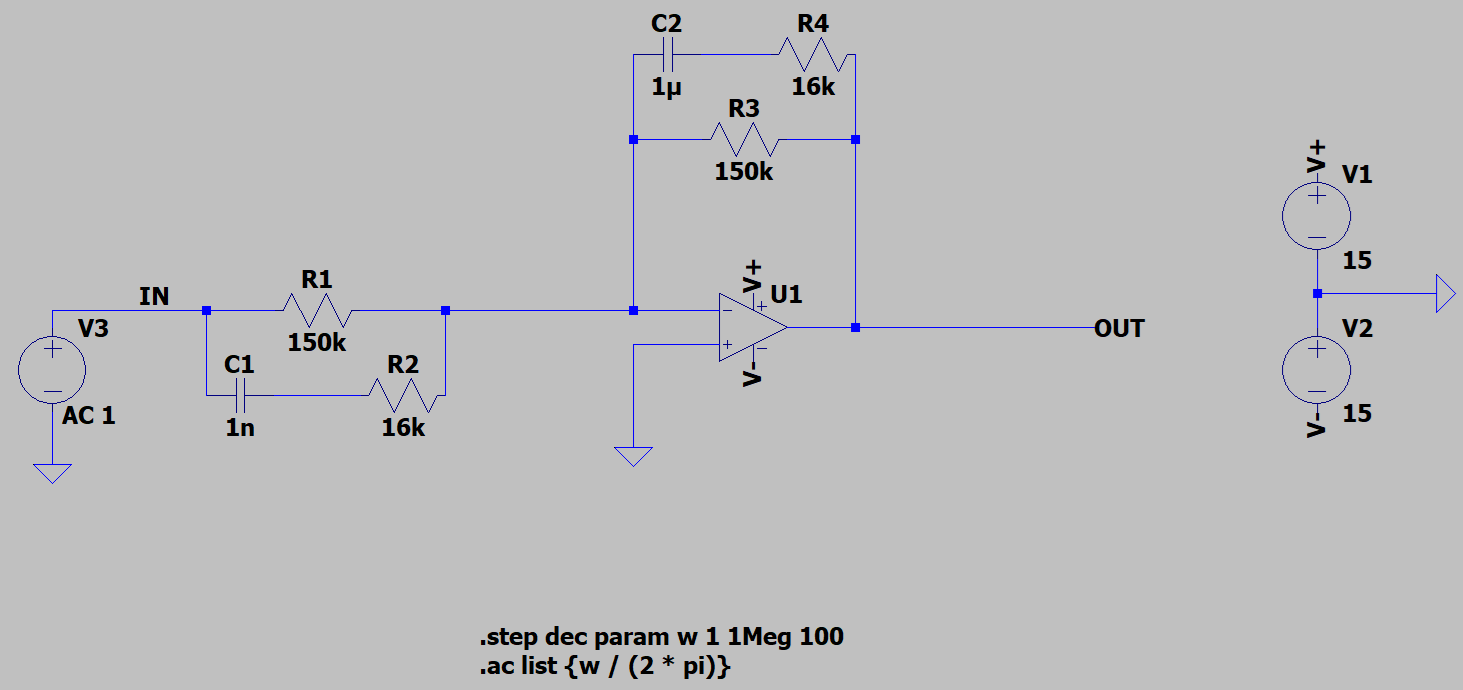
\includegraphics[width=0.8\textwidth]{Schematic.png}
    \caption{Aufgebaute Schaltung}
    \label{fig:SchaltungInLTSpice}
\end{figure}

\begin{figure}[htbp]
    \centering
    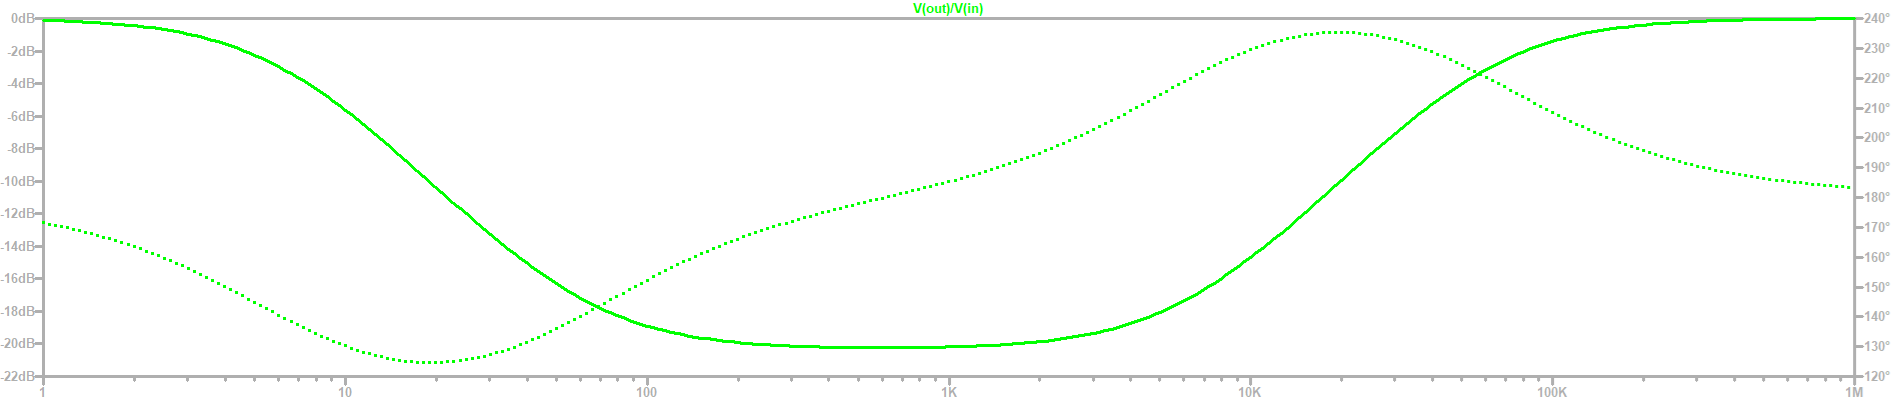
\includegraphics[width=0.8\textwidth]{Frequenz und Phasengang.png}
    \caption{Frequenz und Phasengang der Schaltung mit den berechneten Bauteilwerten}
    \label{fig:Frequenz-Phasengang}
\end{figure}
% ============================================================
\section{Aufgabe 4: Sprungantwort (LTSpice)}
% ============================================================
 
\subsection{Laplace-Analyse der Sprungantwort}
 
Das Eingangssignal ist ein Sprung der Höhe $u_e = -1\,\text{V}$ bei $t = 0$:
\[
  U_e(s) = \frac{-1}{s}
\]
 
Das Ausgangssignal im Laplace-Bereich:
\[
  U_a(s) = T(s) \cdot U_e(s)
          = -\frac{R_3}{R_1}
            \cdot \frac{1 + sC_2 R_4}{1 + sC_2(R_3+R_4)}
            \cdot \frac{1 + sC_1(R_1+R_2)}{1 + sC_1 R_2}
            \cdot \frac{-1}{s}
\]
 
Das System hat zwei Pole (bei $s = -\omega_1$ und $s = -\omega_3$), zwei Nullstellen
(bei $s = -\omega_2$ und $s = -\omega_4$) sowie den Pol bei $s = 0$ vom Eingangssprung.
 
\subsection{Zeitkonstanten und stationärer Endwert}
 
Die zwei Systemzeitkonstanten entsprechen den Polen:
 
\begin{align*}
  \tau_1 &= \frac{1}{\omega_1} = \frac{1}{62} \approx 16{,}1\,\text{ms}
  \qquad \text{(Pol von } Z_1\text{, langsame Zeitkonstante)} \\[4pt]
  \tau_2 &= \frac{1}{\omega_3} = \frac{1}{6200} \approx 161\,\mu\text{s}
  \qquad \text{(Pol von } Z_2\text{, schnelle Zeitkonstante)}
\end{align*}
 
Stationärer Endwert ($t \to \infty$, entspricht $s \to 0$):
\[
  u_a(\infty) = \lim_{s \to 0}\; s \cdot U_a(s)
              = T(0) \cdot (-1)
              = -\frac{R_3}{R_1} \cdot (-1)
              = \frac{15\,\text{k}}{150\,\text{k}}
              = +0{,}1\,\text{V}
\]
 
\begin{tcolorbox}[hinweis, title=Erwartetes Verhalten der Sprungantwort]
\begin{enumerate}
  \item \textbf{Initialer Sprung} (D-Anteil, $t = 0^+$): Der Zähler-Term
        $(1 + sC_2R_4)$ bewirkt einen starken Ausschlag direkt beim Sprung.
        Der Ausgangswert springt instantan auf:
        \[
          u_a(0^+) = T(\infty) \cdot (-1) = -0{,}1\,\text{V}
        \]
  \item \textbf{Exponentieller Abfall} (P-/I-Anteil): Die zwei Zeitkonstanten
        $\tau_1 \approx 16\,\text{ms}$ und $\tau_2 \approx 161\,\mu\text{s}$ bestimmen
        das Abklingverhalten.
  \item \textbf{Stationärer Endwert}: $u_a(\infty) = +0{,}1\,\text{V}$
\end{enumerate}
\end{tcolorbox}
 
\subsection{LTSpice: Transientenanalyse}
 
\begin{verbatim}
.tran 0 30ms 0 1us
\end{verbatim}
 
Eingangsspannung als Pulsquelle (idealer Sprung):
\begin{verbatim}
PULSE(0 -1 0 1ns 1ns 30ms 60ms)
\end{verbatim}
 
\begin{itemize}
  \item Simulationszeit: $30\,\text{ms}$ (deckt $\approx 2\tau_1$ ab)
  \item Sprunghöhe: $u_e = -1\,\text{V}$
  \item Maximale Schrittweite: $1\,\mu\text{s}$ (ausreichend für $\tau_2 = 161\,\mu\text{s}$)
\end{itemize}
 
% ============================================================
\section{Zusammenfassung}
% ============================================================
 
\begin{table}[H]
  \centering
  \caption{Zusammenfassung aller Ergebnisse}
  \begin{tabular}{ll}
    \toprule
    Größe & Ergebnis \\
    \midrule
    $T(s)$ &
      $-\dfrac{R_3}{R_1}\cdot\dfrac{1+sC_2R_4}{1+sC_2(R_3+R_4)}\cdot\dfrac{1+sC_1(R_1+R_2)}{1+sC_1R_2}$ \\[8pt]
    $C_1$ & $100\,\text{nF}$ \\
    $C_2$ & $10\,\text{nF}$ \\
    $R_1$ & $150\,\text{k}\Omega$ \\
    $R_2$ & $16\,\text{k}\Omega$ \\
    $R_3$ & $15\,\text{k}\Omega$ \\
    $R_4$ & $1{,}6\,\text{k}\Omega$ \\
    $\omega_1$ & $62\,\text{rad/s}$ (Pol, $-20\,\text{dB/Dek.}$) \\
    $\omega_2$ & $620\,\text{rad/s}$ (Nullstelle, $+20\,\text{dB/Dek.}$) \\
    $\omega_3$ & $6200\,\text{rad/s}$ (Pol, $-20\,\text{dB/Dek.}$) \\
    $\omega_4$ & $62000\,\text{rad/s}$ (Nullstelle, $+20\,\text{dB/Dek.}$) \\
    $|T(0)|$ & $0{,}1$ \\
    $|T(\infty)|$ & $0{,}1$ \\
    $u_a(\infty)$ bei $u_e = -1\,\text{V}$ & $+0{,}1\,\text{V}$ \\
    $\tau_1$ & $\approx 16{,}1\,\text{ms}$ \\
    $\tau_2$ & $\approx 161\,\mu\text{s}$ \\
    \bottomrule
  \end{tabular}
\end{table}
 
% ============================================================
\section*{Anhang: LTSpice Netzliste}
% ============================================================
\addcontentsline{toc}{section}{Anhang: LTSpice Netzliste}

Spice Netliste für AC Analyse 
\begin{verbatim}
V1 V+ 0 15
V2 0 V- 15
R1 N002 IN 150k
R2 N002 N003 16k
X§U1 0 N002 V+ V- OUT level1 Avol=1Meg GBW=1G Vos=0 En=0 Enk=0 In=0 Ink=0 Rin=500Meg
C1 N003 IN 1n
R3 N002 OUT 150k
R4 N001 OUT 16k
C2 N002 N001 1µ
V3 IN 0 AC 1
.step dec param w 1 1Meg 100
.ac list {w / (2 * pi)}
.lib UniversalOpAmp1.lib
.backanno
.end
\end{verbatim}

Spice Netliste für Sprungantwort

\begin{verbatim}
V1 V+ 0 15
V2 0 V- 15
R1 N002 IN 150k
R2 N002 N003 16k
X§U1 0 N002 V+ V- OUT level1 Avol=1Meg GBW=1G Vos=0 En=0 Enk=0 In=0 Ink=0 Rin=500Meg
C1 N003 IN 1n
R3 N002 OUT 150k
R4 N001 OUT 16k
C2 N002 N001 1µ
V3 IN 0 AC 1
.step dec param w 1 1Meg 100
.ac list {w / (2 * pi)}
.lib UniversalOpAmp1.lib
.backanno
.end
\end{verbatim}
 
\end{document}